

%%%%%%%%%%%%%%%%%%%%%%%%%%%%%%%%%%%%%%%%%%%%%%%%%%%%%%%%%%%%%%%%%%%%%%%%%%% START OF INTRODUCT SECTION %%%%%%%%%%%%%%%%%%%%%%%%%%%%%%%%%%%%%%%%%%%%%%%%%%%%%%%%%%%%%%%%%%%%%%%%
\section{Introduction}
\label{sec:intro}

\begin{framed}
\xxxxn{TODO Notes from Proposal Defense:}
\begin{itemize}
        \item \xxxxn{Motivation regarding alternative solutions: private vs public network, separate networks for control and grid itself, power link communication.  need
to motivate having a separate network and that generic routers are insufficient.} 
        \item \xxxxn{2 types of Backup Computations: (1) initialization, and (2) after each link failure } 
        \item \xxxxn{Including writing about efficient implementation of algorithms using OpenFlow } 
        \item \xxxxn{Mention in future work about simultaneous link failures: the input to the new version of each algorithm will now take a vector of links, instead of a single link. }
		\item \xxxxn{Distinguish between link failure, packet loss, packet delay + be consistent with terminology.}
\end{itemize}
\end{framed}
               

An electric power grid consists of a set of buses  -- electric substations, power generation centers, or aggregation points of electrical loads -- and transmission lines connecting those buses.
The operation of the power grid can be greatly improved by high-frequency voltage and current measurements. Phasor Measurement Units (PMUs) are  
sensors that provide such measurements. PMUs are currently being deployed in electric power grids worldwide, providing the potential to both 
(a) drastically improve existing power grid operations and applications and (b) enable an entirely new set of applications,
such as real-time visualization of electric power grid dynamics and the reliable integration of renewable energy resources. 

PMU applications have stringent and in many cases ultra-low \emph{per-packet} delay and loss requirements.  
If these per-packet delay requirements are not met, PMU applications can miss a critical power grid event (e.g., lightning strike, power link failure), potentially leading to a 
cascade of incorrect decisions and corresponding actions. For example, closed-loop control applications require delays of $8-16$ ms per-packet \cite{Bakken11}. 
If \emph{any} packet is not received within this time window, the closed-loop control application may take a wrong control action.
In the worst case, this can lead to a cascade of power grid failures (e.g., the August 2003 blackout in the USA 
\footnote{\url{http://en.wikipedia.org/wiki/Northeast\_blackout\_of\_2003}} and the recent power grid failures in India \cite{IndiaBlackout}). 


As a result of this sensitivity, the communication network that disseminates PMU data must provide hard end-to-end data delivery guarantees \cite{Bakken11}. 
For this reason, the Internet's best-effort service model alone is unable to meet the stringent packet delay and loss requirements of PMU applications \cite{Birman05}. 
Instead, either a new network architecture or enhancements to Internet architecture and protocols are needed \cite{Bakken11,Birman05,Naspi10,Hopkinson09} to provide efficient, in-network forwarding and fast recovery from link and switch failures. 
Additionally, multicast should figure prominently in data  delivery, since PMUs disseminate  data  to applications across many locations \cite{Bakken11}.

In this last piece of our research, we design algorithms for fast recovery from link failures in a Smart Grid communication network. 
Informally, we consider a link that does not meet its packet delivery requirement (either due to excessive delay or actual packet loss) as failed.  Our proposed research divides broadly into two parts:
\begin{itemize}
	
	\item {\bf Link detection failure.} 
		Here, we design link-failure detection and reporting mechanisms that use OpenFlow \cite{OpenFlow08} -- an open source framework that centralizes network management and control -- 
		to detect link failures when and where they occur, \emph{inside} the network.  In-network detection is used to reduce the time between when the loss occurs and when it is detected. 
		In contrast, most previous work \cite{Almes99,Caceres99,Friedl09} focuses on measuring end-to-end packet loss, resulting in slower detection times. 

	\item {\bf Algorithms for pre-computing backup multicast trees.} 
		Inspired by MPLS fast-reroute algorithms that are used in practice to quickly reroute time-critical unicast IP flows over pre-computed backup paths \cite{Cui04,Fei01,Medard99,Pointurier02,Wu97}, 
		we propose a set of algorithms, each of which computes backup multicast trees that are installed after a link failure. We also implement these algorithms in OpenFlow and demonstrate their performance.
		
		Each algorithm computes backup multicast trees that aim to minimize end-to-end packet loss and delay, but each algorithm uses different optimization criteria in achieving this goal: 
		minimizing control overhead (\mcs), minimizing \xxn{the maximum number of flows impacted by the ``next'' link failure (\mfs)},
   		and minimizing \xxn{the maximum number of sink nodes impacted by the ``next'' link failure (\mds)}.  These optimization criteria differ from those proposed in the literature.
		For example, most previous work \cite{Cui04,Fei01,Medard99,Pointurier02,Wu97} uses optimization criteria specified over a \emph{single} multicast tree, while we must consider 
		criteria specified across \emph{multiple} multicast trees. Finally, because the smart grid network is many orders of magnitudes smaller than the Internet
		\footnote{For example, it is estimated that fewer than $10^4$ routers/switches are needed for a smart grid network spanning the \emph{entire} USA, whereas there are about $10^8$ routers in the Internet \cite{Bakken11}.} 
		and multicast group membership is mostly static in the Smart Grid, we can for the most part avoid the scalability issues of Internet-based solutions \cite{Cui04,Fei01,Medard99,Pointurier02,Wu97}.

\end{itemize}


The remainder of this chapter is structured as follows.  In the following section (Section \ref{sec:background}), we provide necessary background on PMU application requirements and OpenFlow.  
Then, we briefly survey relevant literature (Section \ref{sec:related}).
We outline proposed research in Section \ref{sec:proposed}:
section \ref{subsec:detection} details our research thus far on link-failure detection in OpenFlow, and in section \ref{subsec:repair}, we outline our algorithms for computing backup multicast trees.
Our treatment here is necessarily brief, but we indicate work completed thus far as well as proposed future work.  Section \ref{sec:conclude} concludes this chapter with a summary of our proposed research and 
timeline for future work.

%%%%%%%%%%%%%%%%%%%%%%%%%%%%%%%%%%%%%%%%%%%%%%%%%%%%%%%%%%%%%%%%%%%%%%%%%%% END OF INTRODUCT SECTION %%%%%%%%%%%%%%%%%%%%%%%%%%%%%%%%%%%%%%%%%%%%%%%%%%%%%%%%%%%%%%%%%%%%%%%%














%%%%%%%%%%%%%%%%%%%%%%%%%%%%%%%%%%%%%%%%%%%%%%%%%%%%%%%%%%%%%%%%%%%%%%%%%%% START OF BACKGROUND/RELATED WORK SECTION %%%%%%%%%%%%%%%%%%%%%%%%%%%%%%%%%%%%%%%%%%%%%%%%%%%%%%%%%%%%%%%%%%%%%%%%

\section{Background}
\label{sec:background}

\subsection{PMU Applications and Their QoS Requirements} 
\label{subsec:pmu-requirements}

The QoS requirements of several PMU applications planned to be deployed on power grids worldwide are presented in Table \ref{tab:app-requirements}, based on \cite{Bakken11,Kth09}.
We refer the reader to the actual documents for a description of each PMU application.  The end-to-end (E2E) delay requirement is at the \emph{per-packet} level, as advocated by
Bakken et al. \cite{Bakken11}.

NASPI defines five service classes (A-E) for Smart Grid traffic, each designating qualitative requirements for latency, availability, accuracy, time alignment, message rate, 
and path redundancy \cite{Bakken11}. At one end of the spectrum, service class A applications have the most stringent requirements, while service Class E designates applications
with the least demanding requirements.

In this work, we focus on PMU applications with the most stringent E2E delay requirements, such as closed-loop control and system protection. 
In particular, we create a binary classification of data plane traffic: traffic belonging to critical PMU applications and all other traffic. 



\begin{table}[t]
\begin{center}
\begin{tabular}{|l|l|l|c|} 
\hline
   	{\bf PMU Application} & {\bf E2E Delay} & {\bf Rate (Hz)} & {\bf NASPI Class} \\ 
		  \hline \hline
		
	%		$\diamondsuit$ Arming Remedial Action  & \textasciitilde $100$ ms & $30$  & N/A \\ 
	%		$\diamondsuit$ Out of Step Protection  & \textasciitilde $100$ ms & $30$  & N/A \\ 
	%		$\diamondsuit$ Short-term Stability Control  & \textasciitilde $100$ ms & $30$  & N/A \\ 
	%		\hline
			$\heartsuit$ Oscillation Detection & $0.25 - 3$ secs & $10-50$  & N/A \\
			$\heartsuit$  Frequency Instability & $0.25-0.5$ secs & $1-50$ & N/A  \\
			$\heartsuit$  Voltage Instability & $1-2$ secs &  $1-50$  & N/A  \\
			$\heartsuit$  Line Temp. Monitoring & $5$ minutes & $1$ & N/A  \\
			\hline
			$\triangle$ Closed-Loop Control & $8-16$ ms & $120-720+$ & A \\ 
			$\triangle$  Direct State Measurement & $5-1000+$ ms & $1-720+$  & B \\
			$\triangle$ Operator Displays & $1000+$ ms & $1-120$ & D \\
			$\triangle$ Distributed Wide Area Control & $1-240$ ms & $1-240$  & B  \\
			$\triangle$ System Protection & $5-50$ ms & $120-720+$  & A  \\
			$\triangle$  Anti-Islanding & $5-50$ ms & $30-720+$  & A  \\
			$\triangle$  Post Event Analysis & $1000+$ ms & $< 1$ & E \\
			\hline
			\end{tabular}
			\end{center}
\caption{PMU applications and their QoS requirements.  The $\heartsuit$ refers to reference \cite{Kth09} and $\triangle$ to \cite{Bakken11}. }
\label{tab:app-requirements}
\end{table}

\xxxx{state than nothing is published regarding tolerance to packet loss.}


\subsection{OpenFlow}
\label{subsec:openflow}

OpenFlow is an open source framework that cleanly separates the control and data planes, and provides a programmable (and possibly centralized) control framework \cite{OpenFlow08}.
All OpenFlow algorithms and protocols are managed by a (logically) centralized controller, 
while network switches/routers (as their only task) forward packets according to the flow tables installed by the controller. 
By allowing a more centralized network control and management framework, the OpenFlow architecture avoids the high storage, computation, and management overhead that plague many distributed network approaches.
Our multicast tree repair algorithms benefit from these OpenFlow features (Section \ref{subsec:repair}).

OpenFlow exposes the flow tables of its switches, allowing the controller to add, remove, and delete flow entries, which determine how switches 
forward, copy, or drop packets associated with a controller-managed flow. 
Phrased differently, OpenFlow switches follow a ``match and action'' paradigm \cite{OpenFlow08}, in which each switch \emph{matches} an incoming packet 
to a flow table table entry and then takes some \emph{action} (e.g., forwards, drops, or copies the packet).
Each switch also maintains per-flow statistics (e.g., packet counter, number of bytes received, time the flow was installed) that can 
can be queried by the controller.  In summary, OpenFlow provides a flexible framework for \emph{in-network} packet loss detection as 
demonstrated by our detection algorithms (Section \ref{subsec:detection}).
%For our detection algorithms, the packet counter statistics are key to our packet loss computations (Section \ref{subsec:detection}). 
%\yyn{Our detection algorithms are also aided by OpenFlow's ability to:  install packet counters at any time and arbitrarily group flows together 
%(this enables network operators to reduce measurement overhead by first installing general matching rules and then drilling down into more detail by installing finer-grained matching rules). }
%Note that because these statistics are maintained \emph{inside} the network (at each switch) and the controller can query any switch for its per-flow statistics, 
%OpenFlow provides the framework for \emph{in-network} packet loss detection.

\xxn{OpenFlow switches can support a limited number of flow entries because they rely on expensive TCAM memory to perform wildcard matching.  
For example, the HP5406zl switch supports approximately $1500$ OpenFlow rules \cite{Curtis11} and the NEC PF5820 switch can handle about $750$ flow entries \cite{PF5820}.
}

\xxn{OpenFlow is similar in spirit to past work in Active Networking \cite{Psounis99}, as both aim to create programmable networks, but is implemented differently.  Active Networking puts the smarts
\emph{inside} the network: customized smart routers are used to interpret and execute commands (that may modify network state) specified in code-carrying packets. 
In contrast, OpenFlow moves the network intelligence (i.e., control logic) \emph{outside} of the network 
and into the controller, while switches become dumb forwarders of data as they simply follow the instructions dictated by the controller.
}

\section{Related Work}
\label{sec:related}

\subsection{Smart Grid Communication Architectures}


The Gridstat project \footnote{\url{http://gridstat.net/}}, started in 1999, was one of the first research projects to consider smart grid communication.  
Our work has benefited from their %requirements elicitation and 
detailed requirements specification \cite{Bakken11}.

Gridstat proposes a publish-subscribe architecture for PMU data dissemination. By design, subscription criteria are simple to enable fast forwarding of PMU data
(and as a measure towards meeting the low latency requirements of PMU applications).  
Gridstat separates their system into a data plane and a management plane. The management plane keeps track of subscriptions,
monitors the quality of service provided by the data plane, and computes paths from subscribers to publishers.  To increase reliability, each Gridstat publisher sends data over multiple paths
to each subscriber. Each of these paths is a part of a different (edge-disjoint) multicast tree.  Meanwhile, the data plane simply forwards data according to the paths and subscription 
criteria maintained by the management plane.  

Although Gridstat has similarities with our work, their project lacks details.  For example, no protocol is provided defining communication between the management and data plane. 
Additionally, there is no explicit indication if the multicast trees are source-based.

In North America, all PMU deployments are overseen by the North American SynchroPhasor Initiative (NASPI) \cite{Naspi10}.  NASPI has proposed and started (as of December 2012) to build the
communication network used to deliver PMU data, called NASPInet. The interested reader can consult \cite{Naspi10} for more details.
%\xxx{Mention: (a) hub-and-spoke architecture, (b) PMU data aggregated by Phasor Data Concentrator, (c) not sure if use multicast? }


Hopkinson et al \cite{Hopkinson09} propose a Smart Grid communication architecture that handles heterogeneous traffic: traffic with strict timing requirements (e.g., protection systems), 
periodic traffic with greater tolerance for delay, and aperiodic traffic. They advocate a multi-tier data dissemination architecture: use a technology such as MPLS to make hard
bandwidth reservations for critical applications, use Gridstat to handle predictable traffic with less strict delivery requirements, and finally use Astrolab (which uses a gossip protocol) 
to manage aperiodic traffic sent over the remaining available bandwidth. They advocate hard bandwidth reservations -- modeled as a multi-commodity flow problem -- for critical Smart
Grid applications.




\subsection{Detecting Packet Loss} 

Most previous work \cite{Almes99,Caceres99,Friedl09} focuses on measuring and detecting packet loss on an end-to-end packet basis.
Because PMU applications have small per-packet delay requirements (Section \ref{subsec:pmu-requirements}), the time delay between when the loss occurs and when it is detected needs to be small.  
For this reason, we will investigate detecting lossy links \emph{inside} the network. 
Additionally, most previous work takes an \emph{active measurement} approach towards detecting lossy links in which probe messages are injected to estimate packet loss.  Injecting packets can
potentially skew measurements -- especially since accurate packet loss estimates require a high sampling probing rate -- leading to inaccurate results \cite{Barford04}. 


Friedl et al. \cite{Friedl09} propose a \emph{passive} measurement algorithm that directly measures actual network traffic to determine application-level packet loss rates. 
Unfortunately, their approach can only measure packet loss after a flow is expired.  This makes their algorithm unsuitable for our purposes because
PMU application flows are long lasting (running continuously for days, weeks, and even years). 
For this reason we propose a new algorithm, \fls, that provides in-network packet loss detection for long running active flows (Section \ref{subsec:detection}).

We note that existing Internet  ??? routing ??? algorithms (e.g., OSPF, ISIS, BGP) perform in-network detection of link failure, but not of individual packet loss. They do so by
having routers exchange ``keep-alive'' or ``hello'' messages and detect a link failure when these messages or their acknowledgments are lost.

\xxn{A standard Internet-based approach to passive monitoring of packet loss is to query the native Management Information Base (MIB) counters stored at each router using Simple Network
Management Protocol (SNMP) \cite{Barford04}. This approach is well suited for course-grained packet loss measurements but not for the fine-grained packet loss detection required
by critical PMU applications.  Specifically, this approach cannot provide synchronized reads of packet counts across routers/switches.}
%We require fine-grained packet loss measurements that this approach cannot support because we consider PMU applications with ultra-low tolerance to packet loss. }
%This approach is better suited for course-grained measurements


%\xxxx{mention shortcomings of SNMP and MIB from \cite{Barford04}.}
%\xxn{A standard approach to passive monitoring of packet loss, especially in lossy environments where passive monitoring using statistical sampling yields poor results, is to query the native ManagementInformation Base (MIB) counters stored at each router using Simple Network Management Protocol (SNMP) \cite{Barford04}.  
%Using a trace-driven empirical analysis, Barford and Sommers \cite{Barford04} find that SNMP-reported packet loss measurements are very accurate. However, the data storage overhead at each router and limited SNMP access across administrative domains makes this approach 
%impractical. Because we use OpenFlow's native packet counters and OpenFlow's standardized protocol to query routers, we are able to implement a system that is practical and provides accurate 
%packet loss measurements.} 


%\xxxx{{\bf (A1)}: mention Rexford paper using OpenFlow.  We leverage their solutions. }

\subsection{Multicast Tree Recovery}

\xxxx{{\bf (B)} mention the multicast recovery approaches that don't use MPLS?}

Approaches to multicast fault recovery can be broadly divided into two groups: on-demand and preplanned. 
In keeping with their best-effort philosophy, most Internet-based algorithms compute recovery paths on-demand \cite{Cui04}. 
Because the Smart Grid is a critical system and its applications have strict delivery requirements, we focus our literature survey instead on preplanned approaches to failure recovery. 
 
To date, most preplanned approaches \cite{Cui04,Fei01,Medard99,Pointurier02,Wu97} are implemented (or suggest an implementation) using 
virtual circuit packet switching, namely, MPLS. \xxn{Citations \cite{Luebben09,Tam09} are exceptions, as they both consider preplanned recovery for link failures affecting basic IP multicast traffic.}
For convenience, in the remainder of this section we assume MPLS is the virtual circuit packet switching technology used, realizing that other such technologies could be used in its place.

Cui et \cite{Cui04} define four categories for preplanned multicast path recovery: (a) link protection, (b) path protection, (c) dual-tree protection, and (d) redundant tree protection.
With link protection, a backup path is precomputed for each link, connecting the link's end-nodes \cite{Pointurier02,Wu97}. 
For each destination, a path protection algorithm computes a vertex-disjoint path with the original multicast tree path between the source and destination \cite{Wu97}. 
The dual-tree approach precomputes a backup tree for each multicast tree. The backup (dual) tree is not required to be node- or link-disjoint with the primary tree but this is 
desirable \cite{Fei01,Tam09}. Lastly, a redundant tree is node (link) disjoint from the primary tree, thereby ensuring that any destination
remains reachable, either by the primary or redundant tree, if any vertex (edge) is eliminated \cite{Medard99}. \xxn{This approach requires link and node disjointedness in the network topology.} 

\xxn{
However, not all previous work fits nicely into this taxonomy.  Li et al. \cite{Li06} and Kodialam et al. \cite{Kodialam02} compute backup paths for each link in the primary tree
connecting the upstream node to each of its downstream nodes in the original primary tree. Our approach (and likewise the work by Tam et al. \cite{Tam09}) does not fall into any of these categories, as
we propose a backup tree be computed for each link in each multicast tree. 
}


{\bf Optimization Criteria.}
Our recovery algorithms use different optimization criteria from previous work considered in this document \cite{Cui04,Fei01,Kodialam02,Lau05,Li06,Luebben09,Medard99,Pointurier02,Wu97}. 
With one exception \cite{Li06} (discussed below) past approaches use local/myopic optimization criteria (i.e., constraints specified over a \emph{single} multicast tree),
while we consider global (network-wide) criteria (i.e., constraints specified across \emph{multiple} multicast trees).  In addition, none of these approaches explicitly optimize
for the criteria we consider: minimizing control overhead, \xxn{minimizing the maximum number of flows impacted by the ``next'' link failure (\mfs)}, and 
\xxn{minimizing the maximum number of sink nodes impacted by the ``next'' link failure (\mds)}.
Instead, previous work computes backup paths or trees that optimize one of the following criteria: maximize node (link) disjointedness with the primary 
path \cite{Cui04,Fei01,Luebben09,Medard99}, minimize bandwidth usage \cite{Wu97}, minimize backup bandwidth reservations \cite{Kodialam02,Lau05,Li06}, minimize the number of group members which become disconnected (using either the primary or backup path) after a link failure \cite{Pointurier02}, or minimize path length \cite{Tian05}.



\xxn{
%Most MPLS-based approaches to link failure recovery, termed ``fast reroute'', focus on unicast flows \cite{??,??}.  In contrast, 
In contrast to other related work, Li et al. \cite{Li06} optimize for criteria spanning several multicast trees: minimizing the \emph{total} bandwidth reserved by backup paths.
Their problem formulation assumes that each source and destination flow is associated with a bandwidth reservation. 
%The authors consider MPLS-based multicast (called point-to-multipoint label switched path) in which it is assumed that each source and destination flow is associated with a bandwidth reservation. 
Under their scheme, backup paths are computed with the goal of minimizing both the restoration time and the total backup bandwidth reserved over \emph{all}
backup paths.  In our research, we also plan to compute backup trees by optimizing for network-wide constraints but we consider criteria other than backup bandwidth reservation. 
%At each node in the tree, a backup path is precomputed to each destination node in the tree. The backup path computed at node $v$ must be disjoint from all links in the tree that are adjacent to $v$.
%A backup path is precomputed between each node in the tree to each destination node.  The backup path is computed at each node  must be  disjoint from any adjacent link in the tree. 
%Backup paths are computed with the goal of minimizing both the restoration time and the total backup bandwidth reservations 
%(network-wide).  In our research, we also plan to compute backup trees by optimizing network-wide criteria but we consider constraints other than bandwidth reservation.
%Their algorithm seeks to maximimize bandwidth sharing among common links, which may span multiple multicast trees.  
}




{\bf Implementation Challenges.}
\xxn{
Each of the protection schemes presented in this section are implemented as distributed algorithms. As a result, each algorithm 
must navigate an inherent trade-off between high overhead and fast recovery (i.e., the time between when the failure is detected and when the
multicast tree is repaired should be small) \cite{Cui04}: preplanned, localized recovery (e.g., fast reroute) is fast but not scalable  while on-demand recovery scales well but can be slow due to
slow convergence time.}
Here, overhead refers to (i) per-router state that needs to be stored and managed and (ii) message complexity associated with the distributed computation.
Because preplanned MPLS-based approaches are tailored to support Internet-based applications -- typically having a large number of multicast groups and dynamic group membership -- scalability is key.
Some of the preplanned approaches (dual-tree and redundant trees) focus more on scalability \cite{Cui04,Fei01,Medard99}, while others 
(link and path protection schemes) optimize for fast recovery \cite{Pointurier02,Wu97}.  

For two reasons, our algorithms avoid these issues of scalability. First,
we use a centralized control architecture (OpenFlow) rather than a distributed one.
Using OpenFlow's centralized architecture, we precompute and store all backup paths (offline) at the controller.  
Thus, we avoid the storage and maintenance issues that distributed approaches must address  \cite{Cui04,Fei01,Pointurier02,Wu97}.
In other words, OpenFlow allows our algorithms to bypass the inherent trade-off of high overhead and fast recovery, allowing (for the first time) both fast \emph{and} scalable recovery algorithms.
\footnote{In the case where the controller is unable to manage router and backup path state, we can simply provision more servers to store precomputed paths.  
Such a situation is unlikely, considering: the encouraging scalability results reported using a centralized Ethane controller \cite{Ethane07} 
(Ethane is a precursor to OpenFlow that also separates the control and data planes), the Smart Grid is many orders of
magnitude smaller that the Internet, and multicast group membership is mostly static in the Smart Grid \cite{Bakken11}.}

Second, the Smart Grid operating environment is very different from the Internet-based applications discussed in the literature.  Specifically, the Smart Grid is many orders of
magnitude smaller that the Internet and Smart Grid multicast group membership is mostly static \cite{Bakken11} (a utility company subscribing to a PMU data stream are likely to always want to
receive updates from this PMU). 


%To activate a precomputed recovery path, the controller simply sends a control message only to the necessary switches, 
%informing the switch to modify its flow table to use the recovery path.  This yields a loose bound of $O(|V|)$ on message complexity.  





\xxn{
%Lastly, 
In the context of OpenFlow, Kotani et al. \cite{Kotani12} propose a clever approach for fast switching between IP multicast trees. 
For reliability purposes, they propose that each multicast group have two multicast trees, a primary tree and a backup tree.
}
\footnote{
	\xxn{
	%Kotani et al \cite{Kotani12} have a simple approach for computing MTs and backup MTs, as this is not the emphasis of their paper.   
	The approach in \cite{Kotani12} for computing MTs and backup MTs is basic, as this is not the emphasis of the paper.   
	The primary and backup tree are both computed using Dijkstra's algorithm \cite{Dijkstra59}.  However, the backup MT is computed over a modified version of the original network, where the 
	link weight of each link in the primary tree is set to infinity, thereby producing link-disjoint trees when possible.
	}
}
\xxn{
Each tree is assigned a unique tree ID and both trees are installed in the network, but only the primary tree is used during normal operation.  
To do so, the root node writes the primary tree ID in each packet header
}
\footnote{Specifically, the tree ID is written in the destination address field of each packet.}
\xxn{, where it is matched and processed by each switch along the primary MT.
}

\xxn{
After a link failure, the root node switches to use the backup tree by writing the backup tree ID in each packet header, 
where it is matched and forwarded by a flow entry at each switch along the backup MT.
Under their approach for failure recovery, only the root node needs to be signaled by the controller to activate a backup tree.  This enables fast switching between the primary and backup MTs.  
We plan to explore this approach as an alternative to the one described in this document: installing backup MTs \emph{after} the link failure is detected. 
}

\xxxx{{\bf A}: something about how the local repairs may eventually lead to a poor overall tree?  Localized for speed, may not be relevant with a centralized controller, more so a concern for distributed
recovery algorithms.}

\xxxx{{\bf A}: ultimately, each of these algorithms requires changes to routers/switches themselves ==> need OpenFlow.}

%\footnote{
%\xxn{
%In more detail, the MT and backup MT computation works as follows.
%The primary MT, $T_1=(V_1,E_1)$, is computed using Dijkstra's algorithm \cite{Dijkstra59} over the input graph $G=(V,E)$, producing an MT that is the union of all shortest paths between 
%the root node and each destination node. 
%Note that this is not the same as computing a Steiner Tree.  The backup MT is also computed using Dijkstra's algorithm but with modified link weights 
%for each link in $T_1$.  For each $e' \in E_1$, $w(e') = 1 + \sum_{\forall e \in E} w(e)$, thereby ensuring that the primary and backup MT are link-disjoint. 
%}
%}




%%%%%%%%%%%%%%%%%%%%%%%%%%%%%%%%%%%%%%%%%%%%%%%%%%%%%%%%%             END RELATED WORK SECTION          %%%%%%%%%%%%%%%%%%%%%%%%%%%%%%%%%%%%%%%%%%%%%%%%%%%%%%%%%%%%%%%%%%%%%%%%%%%%%%%%%%%%%%%%%













%%%%%%%%%%%%%%%%%%%%%%%%%%%%%%%%%%%%%%%%%%%%%%%%%%%%%%%%%%%%%%%%%%%%%  START OF PROPOSED RESEARCH SECTION %%%%%%%%%%%%%%%%%%%%%%%%%%%%%%%%%%%%%%%%%%%%%%%%%%%%%%%%%%%%%%%%%%%%%%%%%%%%%%%%%%%%%%%%%%
\section{Proposed Research}
\label{sec:proposed}

In this section, we present an example problem scenario (Section \ref{subsec:scenario}), which we reference to explain: our link failure detection algorithm (Section \ref{subsec:detection}),
steps to uninstall trees that become disconnected after a link failure (Section \ref{subsec:uninstall-install}), steps to install backup multicast trees (Section \ref{subsec:uninstall-install}),
and our algorithms for computing backup multicast trees (Section \ref{subsec:repair}).




%%%%%%%%%%%%%%%%%%%%%%%%%%%%%%%%%%%%%%%%%%%%%%%%%%%%%%%%%%%%%%%%%%%%%  START OF PROBLEM SCENARIO SECTION %%%%%%%%%%%%%%%%%%%%%%%%%%%%%%%%%%%%%%%%%%%%%%%%%%%%%%%%%%%%%%%%%%%%%%%%%%%%%%%%%%%%%%%%%%


%\subsection{Problem Scenario, Assumptions, and an Example}
%\subsection{Example, Problem Scenario, and Basic Notation}
\subsection{Preliminaries} 
\label{subsec:scenario}

%{\bf Example Scenario}
\subsubsection{Example Scenario}

%Here we present an example problem scenario used Section \ref{subsec:detection} and \ref{subsec:repair} to describe our algorithms.
Figure \ref{fig:intuition-example} depicts a scenario where a single link, $(b,c)$, in a multicast tree fails.  %Figure \ref and the resulting repaired tree.
Figure \ref{fig:intuition-example-t1} shows a multicast tree rooted at $a$ with leaf nodes (i.e., data sinks) $\{e,f,g\}$.  $a$ sends PMU data at a fixed rate and each data sink specifies a per-packet delay requirement. 
The multicast tree in Figure \ref{fig:intuition-example-t1} uses link $(b,c)$, which  we assume fails between the time the snapshots in Figure \ref{fig:intuition-example-t1} and Figure \ref{fig:intuition-example-t2} are taken.
When $(b,c)$ fails, it prevents $e$ and $f$ from receiving any packets until the multicast tree is repaired, leaving $e$ and $f$'s per-packet delay requirements unsatisfied. 
Figure \ref{fig:intuition-example-t2} shows a backup multicast tree installed after $(b,c)$ fails.  Notice that the backup tree does not contain any paths using the failed link, $(b,c)$, and has a path between the root ($a$) and each data sink ($\{e,f,g\}$).  
In the coming sections we present algorithms that allow multicast trees, such as the one shown in Figure \ref{fig:intuition-example-t1}, to recover from link failures by installing backup multicast trees, similar to the one in Figure \ref{fig:intuition-example-t1}.
%In the coming sections we present algorithms that allow the network to recover from scenarios like this one. 

\begin{figure}[t]
  \begin{center}
    \subfigure[Before link $(b,c)$ fails.]{\label{fig:intuition-example-t1}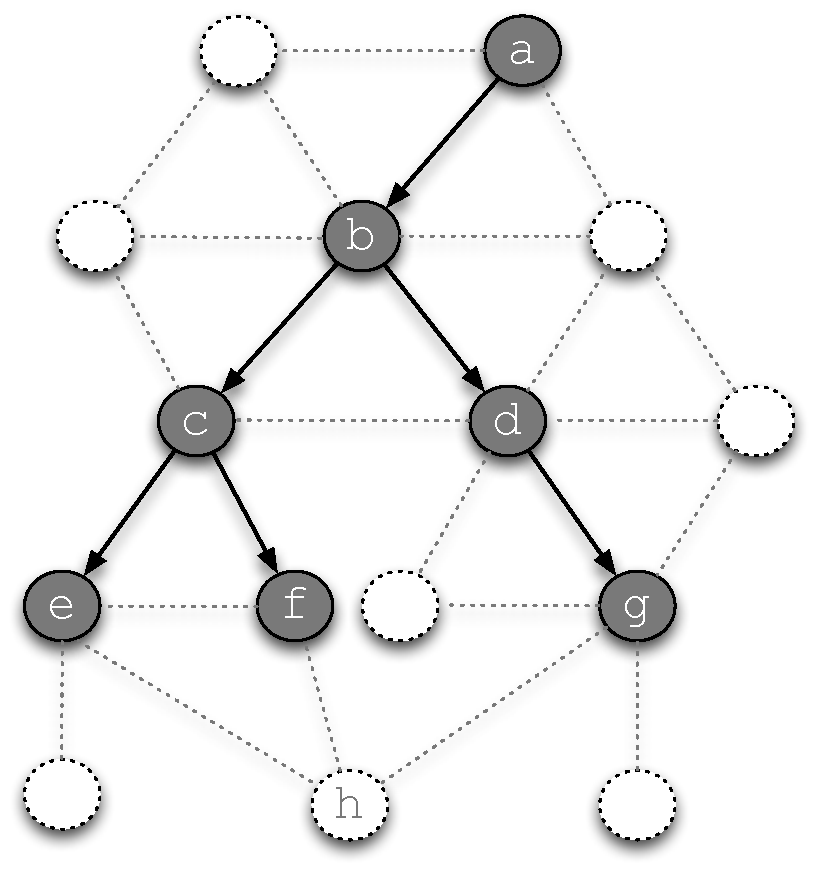
\includegraphics[scale=0.49]{figs/intuition-example-t1.pdf}} 
    \subfigure[After link $(b,c)$ fails.]{\label{fig:intuition-example-t2}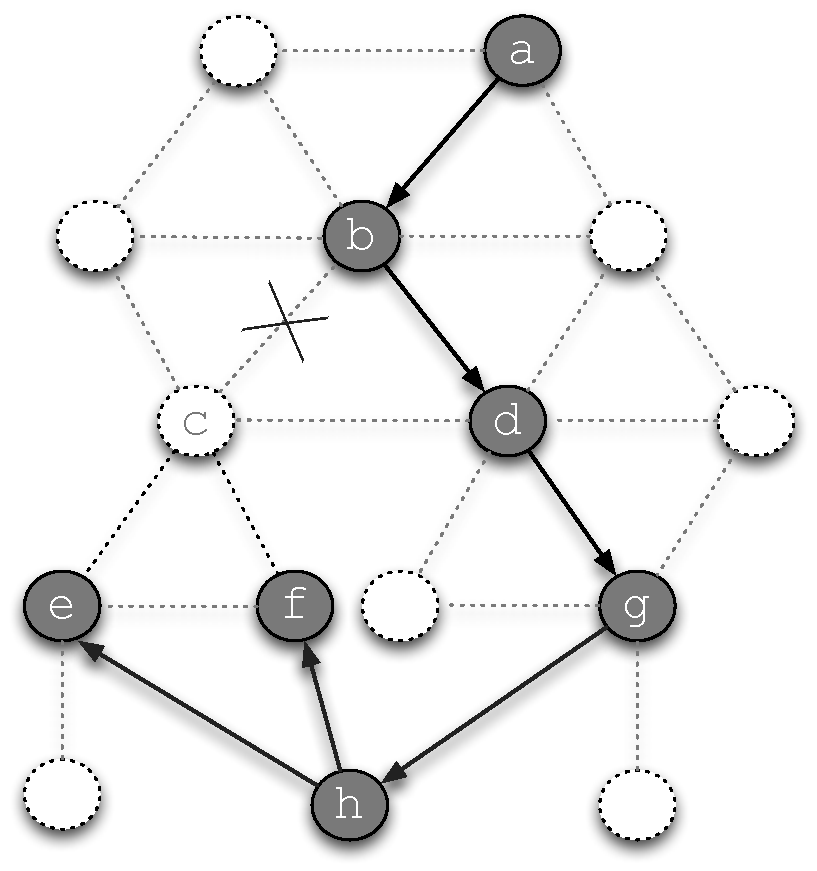
\includegraphics[scale=0.49]{figs/intuition-example-t2.pdf}} 
  \end{center}
\caption{Example used in Section \ref{subsec:mdr}.  The shaded nodes are members of the source-based multicast tree rooted at $a$.  The lightly shaded nodes are not a part of the multicast tree.}
\label{fig:intuition-example}
\end{figure}


\subsubsection{General Problem Scenario and Basic Notation}
\label{subsubsec:mcast-scenario-notation}

Before presenting our algorithms, we first provide a more general problem scenario than the one in Figure \ref{fig:intuition-example} and introduce some basic notation.
We consider a network of nodes modeled as an undirected graph $G=(V,E)$.  There are three types of nodes:
nodes that send PMU data (PMU nodes), nodes that receive PMU data (data sinks), and switches connecting PMU nodes and data sinks (typically via other switches).
We assume $G$ has $m>1$ source-based multicast trees to disseminate PMU data.  Let $T = \{T_1,T_2, \dots T_m\}$, such that each $T_i = (V_i,E_i) \in T$ is a source-based multicast tree (MT). 
We assume $G$ only contains MTs in $T$. 

Each PMU node is the source of its own MT and each data sink has a per-packet delay requirement, specified as the maximum tolerable per-packet delay. 
\emph{Packet delay} between a sender, $s$, and receiver, $r$, is the time it takes $s$ to send a packet to $r$.  
We consider any packet received beyond the maximum delay threshold as lost. Note that a data sink's per-packet delay requirement is an end-to-end requirement.
Before any link fails, we assume that all PMU data is correctly delivered such that each data sink's per-packet delay requirement is satisfied. 

Data sent from a single sender and single data sink is called a \emph{unicast flow}.
A unicast flow is uniquely defined by a four-tuple of source address, source port, destination address, and destination port.  
We assume that data from a single PMU maps to a single port at the source and, likewise, a unique port at the destination. 

Because the network supports multicast communication, \emph{multicast flows} (as opposed to unicast flows) are used inside the network.  
Informally, a multicast flow contains multiple unicast flows and only sends a single packet across a link. 
We use notation $s,\{d_1,d_2, ... d_k\}$ to refer to a multicast flow containing $k$ unicast flows with source, $s$, and data sinks $d_1, d_2, ... d_k$.  The unicast flows are between $s$ and each $d_1, d_2, ... d_k$.
%We use notation $s,\{d_1,d_2, ... d_k\}$ to refer to a multicast flow containing $k$ unicast flows (each denoted $s,d_1$, $s,d_2$, $\dots$, $s,d_k$) with source, $s$, and data sinks $d_1, d_2, ... d_k$.
Each multicast flow, $f = s,\{d_1,d_2, ... d_k\}$, has $k$ end-to-end per-packet delay requirements, one for each of $f$'s data sinks. %each specified by the data sink of each of $f$'s unicast flows.
Let $F$ be the set of all multicast flows in $G$. 
%\yy{Additionally, a multicast flow, $f_m$, sends packets at the maximum rate of the downstream sink nodes among the unicast flows $f_m$ represents. }


We define multicast flows inductively using $T_i \in T$.  Starting at the source/root, $s$, $T_i$ has a multicast flow for each of $s$'s outgoing links $(s,x) \in T_i$. 
For link $(s,x)$ between $s$ and its one-hop neighbor $x$, the multicast flow contains all $T_i$ unicast flows that traverse $(s,x)$. % and have a downstream sink node in $T_i$.
For example, the Figure \ref{fig:intuition-example-t1} multicast tree has a single multicast flow ($a,\{e,f,g\}$) at $a$.   Only a single multicast flow is needed
because $a$ has only one outgoing link in its multicast tree.   
%In the Figure \ref{fig:intuition-example-t1} example, the root node, $a$, only creates a single multicast flow $a,\{e,f,g\}$, because $a$ has only one outgoing link in its multicast tree.   

At internal $T_i$ nodes, additional multicast flows are instantiated when $T_i$ branches.  %In the same way a multicast flow is split at $r$,
Internal node $v \in T_i$, instantiates a new multicast flow for each of $v$'s outgoing links (except for the link connecting $v$ with its parent node in $T_i$).  For outgoing link $(v,u) \in T_i$, 
$v$'s newly instantiated multicast flow represents $T_i$'s unicast flows that traverse $(v,u)$.  In Figure \ref{fig:intuition-example-t1}, the $a,\{e,f,g\}$ flow 
splits when the tree branches at $b$ into multicast flows $a,\{e,f\}$ and $a,\{g\}$.  Likewise, multicast flow $a,\{e,f\}$ splits into multicast flows $a,\{e\}$ and $a,\{g\}$ at $c$.

%OpenFlow does not explicitly provide a multicast implementation, rather, in keeping with its role as a general framework providing necessary services for programmable networks,
In keeping with its role as a general framework providing necessary services for programmable networks, OpenFlow does not explicitly provide an implementation for multicast and multicast flows.
Our initial plan was to use the group table abstraction described in the OpenFlow 1.1 specification \cite{OpenFlowSpec1.1} to implement multicast but, unfortunately,
as of the writing of this paper, this feature is not yet supported by the POX controller \footnote{\url{https://github.com/noxrepo/pox}} used to implement our algorithms and 
the Mininet \footnote{\url{http://mininet.org/}} emulator used in our simulations.  Instead, we assign a multicast IP address to each multicast group and use this abstraction to setup 
the flow tables at the multicast tree switches. Because multicast group membership is static in our power grid application (Section \ref{subsec:pmu-requirements}, 
we simply determine the members of each multicast group by reading their static assignment from a text file.  Note that if dynamic group membership were to be required, we could 
replace this static policy using a protocol like IGMP. 

As with any unicast flow, each switch matches a multicast packet using the {\tt(src\_ip,dst\_ip)} tuple.  If the multicast tree branches, the switch copies the packet 
to be sent out along each of the switch's outgoing links in the multicast tree.  This how the concept of ``splitting''  a flow (introduced in the previous paragraph) is implemented.
If a switch is adjacent to a downstream host in the multicast group, the switch rewrites the destination layer 2 and 3 addresses to those of its adjacent downstream hosts 
(these fields were previously populated with the multicast addresses). 

Another way to implement multicast in OpenFlow is to leverage existing IP multicast protocols as detailed by Kotani et al. \cite{Kotani12}.  
In this approach, the controller assigns a unique group ID to each multicast tree and creates a group table entry, that uses the group ID, at each switch along the multicast tree.  
Meanwhile, the sender and its first-hop switch use IGMP to set up and manage the controller-generated group IDs. Finally, the sender embeds the group ID in each multicast packet's destination 
field, allowing for each switch in the multicast tree to identify and forward multicast packets appropriately. 

%The OpenFlow controller implements multicast flows by creating the appropriate flow entries at each switch along a multicast tree.  
%For a switch $s \in T_i$ with multiple outgoing links in $T_i$, the controller creates a flow entry, $e$, with the following action instructions.
%For each incoming packet satisfying $e$'s match rule, create a copy of the incoming packet for each downstream branch. 
%Then, $e$'s action instruction sends a copy of the packet along each outgoing link (except for the link the original packet arrived on).  This is how a multicast flow is ``split'' (as discussed above).
%In contrast, for $T_i$ switches with only one outgoing link connected to a downstream node, the controller installs a standard flow entry (i.e., one that does not create packet copies),
%as specified in Section \ref{subsec:openflow}. For more details about OpenFlow's multicast implementation, we refer the interested reader to the ``group table'' description in Section 4.2 of OpenFlow Switch Specification Version 1.1.0 \cite{OpenFlowSpec1.1}.

We consider the case where multiple links fail over the lifetime of the network but assume that only a \emph{single link fails at-a-time}.
We call the current lossy or faulty link, $\ell$.  When $\ell$ fails, all sink nodes corresponding to any multicast flow that traverses $\ell$ no longer receive packets from the source. 
As a result, the per-packet delay requirements of each these data sinks is not met. 
We refer to these data sinks, multicast flows, and the MT associated with each such flow %and the corresponding data sinks 
as \emph{directly affected}.  In Figure \ref{fig:intuition-example}, $a,\{e,f\}$ is directly affected by $(b,c)$ failing, along with data sinks $e$ and $f$.

%With one exception, the remaining sections give a myopic presentation of the problem scenario and algorithms; we only detail the effects related to \emph{single} link failure.
%At the end of the section, we briefly comment on how our multicast tree repair algorithms 
%might tailor their reconfiguration to account for \emph{future} link failures. 


%\subsubsection{Overview of Our Recovery Solutions and Section Outline}
\subsection{Overview of Our Recovery Solutions and Section Outline}
\label{subsec:mdr}

%Our approach to making multicast trees robust to link failures divides into three parts: 
We propose an algorithm, \mdrs, that is run at the OpenFlow controller to make multicast trees robust to link failures by monitoring and detecting failed links, precomputing backup multicast trees, and installing backup multicast trees after a link failure.
\footnote{The name \mdr is inspired by Johnny Appleseed, the famous American pioneer and conservationist known for planting apple nurseries and caring for its trees. }
As input, \mdr is given an undirected graph containing OpenFlow switches; the set of all multicast trees ($T$); the set of all active multicast flows ($F$); the length of each sampling window, 
$w$, used to monitor links and specified in units of time; and, for each multicast flow, a packet loss condition for each link the flow traverses. For now, we restrict packet loss conditions 
to be threshold-based that indicate the maximum number of packets that can be lost over $w$ time units. 
The output of \mdr is a new set of precomputed backup multicast trees installed in the network and a set of uninstalled multicast trees.   All $T_i \in T$ that use the failed link are uninstalled and we call each such $T_i$ a \emph{failed multicast tree}.
%The set of installed MTs includes each $T_i \in T$ that does not use the failed link and a backup tree for any $T_i$ that does. %does use a failed link.

We define a \emph{backup multicast tree} for link $\ell$ and $T_i \in T$ as a multicast tree that has 
a path between the source, $s \in T_i$, and each data sink $d \in T_i$ that: (a) connects $s$ and $d$ but does not traverse $\ell$ and 
(b) satisfies $d$'s per-packet delay requirements.  We refer to any multicast tree that satisfies these conditions for $\ell$ a \emph{backup multicast tree for $\ell$} or backup MT for short.
In Figure \ref{fig:intuition-example-t2}, notice that the installed backup tree has paths $a \rightarrow b \rightarrow d \rightarrow g \rightarrow h \rightarrow \{e,f\}$ connecting $a$ with $\{e,f,g\}$ after $(b,c)$ fails.




\mdr divides into three parts: 
\begin{enumerate}
	\item Monitor to detect link failure (e.g., $(b,c)$ in Figure \ref{fig:intuition-example}).
	\item Uninstall all trees using the failed link (i.e., failed trees) and install a precomputed backup multicast tree for each uninstalled tree. 
	For each data sink that was disconnected from the root because of the link failure, the
	 backup tree should use a path that routes around the failed link. 
	 Note that the newly installed tree will likely require changes to several switches upstream from $\ell$, in addition to those at the upstream and downstream ends of link $\ell$.
	 %Note that the newly installed tree will likely require changes at switches in addition to those at the upstream and downstream ends of link $\ell$.
	 Recall in the Figure \ref{fig:intuition-example} example, data sinks $\{e,f\}$ are reconnected with $a$ in the installed backup tree.

	 %backup tree installed and shown in Figure \ref{fig:intuition-example-t2}).
	
	\item Part (2) triggers the computation of a new backup tree for each (backup) tree installed in (2).  % In Section \ref{subsec:repair}, we present three algorithms for computing backup trees: \mcs, \mfs, and \mds.
\end{enumerate}
\mdr uses an OpenFlow-based subroutine (\fls) for part (1) and is presented in Section \ref{subsec:detection}.  For part (2), we briefly describe \mdrs's steps to uninstall and install multicast trees in Section \ref{subsec:uninstall-install}. 
In Section \ref{subsec:repair}, we address part (3)  by proposing a set of algorithms that compute backup multicast trees. 
%We present an OpenFlow-based approach for (1) and (2) in Section \ref{subsec:detection}. In Section \ref{subsec:repair}, we propose a set of algorithms addressing (3).


%Before moving on to present our algorithms, we remind the reader that we divide the problem of making multicast trees robust to link failures into three parts:
%\begin{enumerate}
%	\item Monitor to detect link failure (\fls, presented in Section \ref{subsec:detection}).
%	\item Deactivate all trees using the failed link and install a precomputed backup multicast tree for each deactivated tree (\fls, presented in Section \ref{subsec:detection}).
%	\item Compute a new backup trees for each (backup) tree installed in Step (2).  In Section \ref{subsec:repair}, we present three algorithms for computing backup trees: \mcs, \mfs, and \mds.
%\end{enumerate}

%Our solutions (detailed in the following two sections) compute the repaired multicast tree like the one in Figure \ref{fig:intuition-example-t2} using a three step process: 
%\begin{enumerate}
%	\item Detect the faulty link (e.g., $(b,c)$).
%	\item Deactivate the old multicast tree and install a precomputed backup multicast tree.  The backup tree has a new path, that routes around the failed link,
%	from the source to each data sink that was disconnected from the root because of the link failure (e.g., $\{e,f\}$).
%	\item Compute a new backup tree after the backup tree from (2) is installed.
	%\item For each data sink that becomes disconnected from the root because of the link failure (e.g., $\{e,f\}$), activate precomputed recovery paths connecting these nodes with the root   
	%(e.g, $a \rightarrow b \rightarrow d \rightarrow g \rightarrow h \rightarrow \{e,f\}$). Each recovery path (defined in Section \ref{subsubsec:notation}) must route around the failed link.
%\end{enumerate}
%We present an OpenFlow-based approach for Step (1) in Section \ref{subsec:detection}. In Section \ref{subsec:repair}, we propose a set of algorithms addressing Step (2) and (3).





%%%%%%%%%%%%%%%%%%%%%%%%%%%%%%%%%%%%%%%%%%%%%%%%%%%%%%%%%%%%%%%%%%%%%  END OF PROBLEM SCENARIO SECTION %%%%%%%%%%%%%%%%%%%%%%%%%%%%%%%%%%%%%%%%%%%%%%%%%%%%%%%%%%%%%%%%%%%%%%%%%%%%%%%%%%%%%%%%%%




























%%%%%%%%%%%%%%%%%%%%%%%%%%%%%%%%%%%%%%%%%%%%%%%%%%%%%%%%%%%%%%%%%%%%%  START OF DETECTION SECTION %%%%%%%%%%%%%%%%%%%%%%%%%%%%%%%%%%%%%%%%%%%%%%%%%%%%%%%%%%%%%%%%%%%%%%%%%%%%%%%%%%%%%%%%%%
\subsection{Link Failure Detection using OpenFlow}
\label{subsec:detection}

%\subsection{Link Failure Detection using OpenFlow}
%\label{subsec:detection}

%missing: (a) openflow match and action, (b) flow-level measurement or packet loss at links

In this section, we propose a simple algorithm (\fls), used by \mdrs, that monitors links \emph{inside} the network to detect any packet loss.  To help explain \fls,
we use the example scenario from Section \ref{subsec:scenario} and refer to a generic multicast tree with an upstream node, $u$, and downstream node, $d$.
%Our presentation of \fl is necessarily brief but we provide additional details in Appendix \ref{subsec:pcnt}.  

\fl is run at the OpenFlow controller and provides accurate packet loss measurements that are the basis for identifying lossy links.
Informally, a lossy link is one that fails to meet the packet loss conditions specified by the controller.  We refer to such a link as \emph{failed}.
Although \mdr is ultimately concerned with meeting the per-packet \emph{delay} requirements of PMU applications, 
we use  packet loss (as opposed to delay) as an indicator for a failed link because OpenFlow provides no native support for timers.

\fl has the same input as \mdrs, specified in Section \ref{subsec:mdr}.
The output of \fl is any link that has lost packets not meeting the packet loss condition of any multicast flow traversing the link. 
In the remainder of this document, we assume all flows are multicast and just use \emph{flow} to refer to a multicast flow, unless otherwise specified.

Recall from Section \ref{subsec:openflow} that each OpenFlow switch maintains a flow table, where each entry contains a match rule 
(i.e., an expression defined over the packet header fields used to match incoming packets) and action 
(e.g., ``send packet out port $2$''). For each packet that arrives at an OpenFlow switch, it is first matched to a flow entry, $e$, based on the packet's header fields; 
then $e$'s packet counter is incremented; and, lastly, $e$'s action is executed on the packet. 
\footnote{Not all switches are necessarily OpenFlow-enabled. In fact, we anticipate that in practice many switches will not support OpenFlow. \fl still works such scenarios, as long as 
the packet counts are taken at OpenFlow switches. For ease of presentation, this section assumes all switches are OpenFlow-enabled.}
\fl uses these packet counter values to compute per-flow packet loss between switches over $w$ time units. 

%pcount(upstream_switch,downstream_switchs,nw_src, nw_dst,window_size) or pcount(upstream_switch,downstream_switchs,flow,window_size) 
\fl uses the subroutine, \pcnts, to measure the packet loss between an upstream node ($u$) and one or more downstream nodes.  For simplicity, we assume only a single downstream node, $d$. 
\pcnt does so on a per-flow basis over a specified sampling window, $w$, 
where $w$ is the length of time packets are counted at $u$ and $d$. For each window of length $w$, \pcnt computes packet loss for a flow $f$, that traverses $u$ and $d$, using the following steps:
\begin{enumerate}
	\item 
	\textbf{At $u$, tags and counts all $f$ packets}.  
	We assume, before any changes are made, $u$ uses flow entry $e$ to match and forward $f$ packets.
	\pcnt creates a new flow entry, $e'$, that is an exact copy of $e$, except that $e'$ embeds a unique identifier (i.e., the tag) in the packet's VLAN Id field.  Let this identifying number
	be $1111$.
	$e'$ is installed with a higher priority than $e$.  In OpenFlow, each flow entry has a corresponding priority specified upon its installation.
	%OpenFlow switches order flow entries based on their specified priority.  
	Incoming packets are matched against flow entries in priority order, with the first matching entry being used. 
	Thus, setting a higher priority for $e'$ than $e$, ensures that $u$ writes $1111$ in the VLAN Id field of all $f$ packets when $e'$ is installed.

	\item
	\textbf{Counts all tagged $f$ packets received at $d$.} \pcnt does so by installing a new flow entry at $d$, $e''$, that matches packets with VLAN Id equal to $1111$. 
	%in based on the VLAN tag applied at $u$.  

	\item 
	\textbf{After $w$ time units, turns tagging off at $u$.} To do so, \pcnt simply switches the priority of $e'$ and $e$ at $u$. 
	\footnote{\xxn{Unfortunately, OpenFlow does not allow a flow's priority to be modified.  As a workaround, we install a copy of $e$ called $e_c$.  We ensure that $e_c$ is given 
	a higher priority than $e'$.  Finally, we delete flows $e$. }}

	\item
	\textbf{Queries $u$ and $d$ for packet counts.} 
	Specifically, the controller uses the OpenFlow protocol to query $u$ for $e'$'s packet count value and $d$'s packet count value for $e''$.
	To ensure that all in-transit packets are considered, \pcnt waits ``long enough'' for in-transit packets to reach $d$, before reading $d$'s packet counter 
	(e.g., time proportional to the average per-packet delay between $u$ and $d$).

	\item
	\textbf{Garbage collection.}
	As a cleanup step delete $e'$ at $u$ and $e''$ at $d$.

	\item 
	\textbf{Computes packet loss.}
	The controller computes packet loss by simply subtracting $e'$'s packet count from $e''$'s. 

\end{enumerate}
In practice, \pcnt executes step (2) before step (1) to ensure that $u$ and $d$ consider the same set of packets.

%execute the actions specified by the first flow entry matching the packet's header

\pcnt introduced minimal overhead.  At $u$ and at each downstream counting switch, a copy of the flow entry corresponding to $f$ is required.  
However, these copies only persist during the duration of each \pcnt interval.


In the Figure \ref{fig:intuition-example} example, the controller uses \fl to measure the packet loss for the $a,\{e,f\}$ flow.  
We assume for link $(b,c)$ and the $a,\{e,f\}$ flow, \fl is given a maximum packet loss threshold of $10$ packets over $w$ time units.
For each sampling window of $w$ time units, \pcnt instructs $b$ to tag and count all packets corresponding to $a,\{e,f\}$. 
At the same time, $c$ is instructed by \pcnt to count the $a,\{e,f\}$ packets tagged by $b$. Then, the controller uses the OpenFlow protocol to query the packet counter values for $a,\{e,f\}$
at $b$ and $c$.  When $(b,c)$ fails, the packet counter at $c$ for $a,\{e,f\}$ no longer increments, causing a violation of $a,\{e,f\}$'s packet loss threshold for $(b,c)$.

\xxx{describe how pcount can reduce the number of necessary measurement points}

%As specified, \fl measures packet loss for each \emph{multicast flow} at each link.  These flow-level measurements may obfuscate aggregate link-level packet loss. For this
%reason, we plan to extend \fl to group flows together to enable \emph{aggregate} packet loss measurements. 
%Because OpenFlow provides native support for grouping flows and maintains packet counters for each 
%group, \fl can be easily extended to group and count packets for any subset of multicast flows traversing the same switch.


\pcnts's approach for ensuring consistent reads of packet counters bears strong resemblance to the idea of \emph{per-packet consistency} introduced by Reitblatt et al.~\cite{Reitblatt11}.
Per-packet consistency ensures that when a network of switches change from an old policy to a new one, that
each packet is guaranteed to be handled exclusively by one policy, rather than some combination of the two policies.  In our case, we use per-packet consistency to ensure that when \pcnt reads
$u$ and $d$'s packet counters, exactly the same set of packets are considered, excluding, of course, packets that are dropped at $u$ or dropped along the path from $u$ to $d$. 

\xxn{\fl is fast because it detects link failures inside the network, rather than on an end-to-end basis.  We plan to quantify how much faster \fl is than end-to-end link failure detection 
techniques.  In addition, \fl allows for link failures to be localized, whereas end-to-end techniques may not provide the necessary insight to identify and isolate the faulty link.
}

%\xxn{Advantage of in-network detection is not just the speed but also it allows us to localize the problematic links.  End-to-end detection does not provide this insight, or at least
%not as directly.}



\xxx{ $e$ matches using tuple $(src,dst,VLAN)$}

\subsubsection{\pcnt Evaluation}

\xxxx{move this section, possibly the E2E discussion to the related work section.}

{\bf Detection using end-to-end measurements.}
An alternative approach to link failure detection is to use end-to-end probes to infer packet loss rates of individual links. C\`{a}ceres et al. \cite{Caceres99} propose a maximum likelihood estimator
for loss rates of internal links based on losses observed by multicast receivers. Their model uses the inherent correlation of packet loss across multicast receivers to improve accuracy 
of their packet loss estimates.  Although impressive accuracy results are reported, the authors' simulations show that about $2000$ end-to-end probe messages are required for packet loss
estimates to converge on the true underlying packet loss rate \cite{Caceres99}.  In our problem setting, packet loss needs to be detected over small windows of time and, unfortunately,
$2000$ messages would correspond to too larger a window of time. For this reason, we deem solutions based on end-to-end measurements a poor match for our problem domain.

{\bf 7/20/13 writing from grant about plans for evaluation.}
To date, we have implemented \pcnt in the POX OpenFlow controller using the Mininet emulator and plan to further evaluate \pcnt by using our POX-based implementation to work with real
OpenFlow switches.  To provide a point of reference, we plan to implement and measure a simple SNMP-based approach for detecting link-level packet loss.  We will quantify the error rate of \pcnt 
and the SNMP-based approach as a function of the sampling window size.  We will also quantify the detection time for \pcnt and the SNMP-based approach as a function of window size. We believe our measurement study will show \pcnt  provides accurate and fast packet loss detection across all sampling window sizes, making it a superior approach for ultra- reliable data dissemination in smart grid networks


%%%%%%%%%%%%%%%%%%%%%%%%%%%%%%%%%%%%%%%%%%%%%%%%%%%%%%%%%%%%%%%%%%%%%  END OF DETECTION SECTION %%%%%%%%%%%%%%%%%%%%%%%%%%%%%%%%%%%%%%%%%%%%%%%%%%%%%%%%%%%%%%%%%%%%%%%%%%%%%%%%%%%%%%%%%%








%%%%%%%%%%%%%%%%%%%%%%%%%%%%%%%%%%%%%%%%%%%%%%%%%%%%%%%%%%%%%%%%%%%%%  END OF DETECTION SECTION %%%%%%%%%%%%%%%%%%%%%%%%%%%%%%%%%%%%%%%%%%%%%%%%%%%%%%%%%%%%%%%%%%%%%%%%%%%%%%%%%%%%%%%%%%















%%%%%%%%%%%%%%%%%%%%%%%%%%%%%%%%%%%%%%%%%%%%%%%%%%%%%%%%%%%%%%%%%%%%%  START OF UNINSTALL/INSTALL SECTION %%%%%%%%%%%%%%%%%%%%%%%%%%%%%%%%%%%%%%%%%%%%%%%%%%%%%%%%%%%%%%%%%%%%%%%%%%%%%%%%%%%%%%%%%%

\subsection{Uninstalling Failed Trees and Installing Backup Trees}
\label{subsec:uninstall-install}

After \fl detects $\ell$'s failure, \mdr uninstalls all MTs that contain $\ell$ (i.e., failed trees) and installs a precomputed backup multicast tree for each of these uninstalled tree. Installing 
backup trees for $\ell$, denoted $T_{\ell}$, triggers the computation of new backup trees.  A backup MT is needed for each $T_j \in T_{\ell}$ and for each of $T_j$'s links.
Here we only explain how MTs are uninstalled and installed and describe some of side effects of doing so. We postpone explaining how backup trees are computed until Section \ref{subsec:repair}.

% (1) uninstall and install: what is done 
% (2) backup tree contains recvoery paths.
% (3) directly and indirectly effected flow.
Uninstalling or installing a multicast tree, $T_i$, is simple with OpenFlow.  The controller sends an instruction to each switch in $T_i$ to remove (add) the flow entry corresponding to $T_i$.
Starting at the root and ending at the leaf nodes, flow entries are removed top-down to prevent $T_i$ traffic from being sent while $T_i$ is being uninstalled. 
In contrast, flow entries are installed bottom-up, starting at the leaf
nodes and finishing at the root.  This ensures that when the root node begins to disseminate data using $T_i$ that all downstream $T_i$ nodes are equipped with the necessary flow entries
to correctly forward $T_i$ traffic.

Increased traffic caused by newly installed backup trees may introduce packet loss to multicast flows that do not traverse $\ell$ but do use a path shared by at
least one switch in a backup MT.  
We refer to these flows as \emph{indirectly affected}. Additionally, we refer to any packet or data sink corresponding to an indirectly affected flow as indirectly affected.
In our Figure \ref{fig:intuition-example} example, $a,\{g\}$ is indirectly affected when the backup MT is installed because the backup MT uses paths 
$a \rightarrow b \rightarrow d \rightarrow g \rightarrow h \rightarrow \{e,f\}$. 

%In contrast, we say a multicast flow is \emph{directly affected} by $\ell$'s failure if the flow uses a path that traverses $\ell$. 
%The data sink and packets corresponding to the directly affected flow are also referred to as \emph{directly affected}. In the Section \ref{subsec:scenario} example, 
%$a,\{e,f\}$ is directly affected by $\ell$ failing, along with data sinks $e$ and $f$.








%More formally, we define directly affected flows, data sinks, and packets as follows.Define set $F_{\ell}$ to be the set of flows using a route that traverses $\ell$.   
%Let $f_{\ell}^i$ be the $i$th flow in $F_{\ell}$, where $p_{\ell}^i$ is the path used by $f_{\ell}^i$. We call the set of all $p_{\ell}^i$, $P_{\ell}$. 
%We say that each $f_{\ell}^i \in F_{\ell}$ is \emph{directly affected} by $\ell$'s failure because each $f_{\ell}^i$ may experience increased packet delay and loss.
%Finally, we refer to any packet in $f_{\ell}^i$ and data sink corresponding to $f_{\ell}^i$ as being \emph{directly affected} by $\ell$ failing. 


%The controller activates a recovery path by modifying the flow table of each switch along this path.
%A consequence of doing so, is that any flow using a path sharing a switch, $s$, with a recovery path may experience transient delay and packet loss when $s$ modifies its flow table to activate the recovery path.  
%Likewise, deactivating a stale path that traverses $\ell$ can introduce delay and packet loss to flows that do not use $\ell$.  
%We call any flow using a path that shares at least one switch used by a recovery path or deactivated path, as \emph{indirectly affected}. 
%\footnote{As future work, we plan to quantify this overhead by taking OpenFlow measurements. }
%Additionally, we refer to any packet or data sink corresponding to an indirectly affected flow as indirectly affected.
%In our Figure \ref{fig:intuition-example} example, the flow from $a$ to $g$ is indirectly affected when the recovery paths 
%($a \rightarrow b \rightarrow d \rightarrow g \rightarrow h \rightarrow \{e,f\}$) are activated. % reconnecting $a$ with $e$ and $f$. 

% to activate the recovery path and/or deactivate the original failed path. }
%\yyn{Ultimately, the transient delay and packet loss when $s$ modifies its flow table to activate the recovery path and/or deactivate the original failed path. }


%A consequence of modifying the flow table for each switch along the recovery path is that flows can be \emph{indirectly affected} if the flow 
%A consequence of modifying the flow table for each switch along the recovery path is that flows can be \emph{indirectly affected} if the flow 
%uses a path containing at least one $s \in S_{\ell}$.  We denote the set of indirectly affected flows as $F_{\ell}'$.  
%Each $f \in F_{\ell}'$ may experience transient delay and packet loss when $s$ modifies its flow table to activate the recovery path and/or deactivate the original failed path. 
%This follows from our assumption that control overhead to activate (deactivate) a path is determined by the time it takes each switch in the path to modify its flow table.
%This follows from our assumption that control overhead to activate a recovery path is determined by the time it takes each switch in the recovery path to modify its flow table.
%Additionally, we refer to any packet or data sink corresponding to a flow in $F_{\ell}'$ as \emph{indirectly affected}.







%%%%%%%%%%%%%%%%%%%%%%%%%%%%%%%%%%%%%%%%%%%%%%%%%%%%%%%%%%%%%%%%%%%%%  END OF UNINSTALL/INSTALL SECTION %%%%%%%%%%%%%%%%%%%%%%%%%%%%%%%%%%%%%%%%%%%%%%%%%%%%%%%%%%%%%%%%%%%%%%%%%%%%%%%%%%%%%%%%%%



















%%%%%%%%%%%%%%%%%%%%%%%%%%%%%%%%%%%%%%%%%%%%%%%%%%%%%%%%%%%%%%%%%%%%%  START OF REPAIR/RECOVERY SECTION %%%%%%%%%%%%%%%%%%%%%%%%%%%%%%%%%%%%%%%%%%%%%%%%%%%%%%%%%%%%%%%%%%%%%%%%%%%%%%%%%%%%%%%%%%

\subsection{Computing Backup Multicast Trees}
 \label{subsec:repair}


Here we present a set of algorithms that compute backup MTs.  \mdr uses these algorithms in two scenarios. First, as a part of system initialization 
where a set of backup MTs are computed for each network link, $l$; \mdr computes a single backup MT for each MT that would be directly affected by $l$'s failure. 
% as part of a preplanned approach to recovery from a link failure

Second, \mdr triggers the execution of backup tree computations after backup trees, $T_{\ell}$, are installed in response to the most recent link failure, $\ell$. 
\mdr reruns the entire computation (as opposed to only computing backup MTs for the newly installed $T_{\ell}$ trees): 
for each network link, $l$, \mdr computes a backup MT for each MT that would be affected if $l$ failed.  
\mdr recomputes \emph{all} backup MTs because installing the $T_{\ell}$ MTs changes how flows are distributed and processed inside the network and, as a result, may
adversely affect flows processed by MTs other than those in $T_{\ell}$.
In other words, backup MTs computed before $\ell$ fails may become stale when the $T_{\ell}$ MTs are installed since the algorithms used to compute them considered an old network state in their optimization.
\emph{We hypothesize that recomputing \emph{all} backup MTs each time a single link fails yields a more survivable data dissemination network than only recomputing
backup MTs for newly installed backup MTs installed in response to the most recent link failure. }%newly installed trees.}
%All backup MTs are recomputed because installing $T_{\ell}$ may modify the network state  (e.g., distribution of flows, disjointedness of MTs, etc) and therefore the currently computed backup MTs risk
%becoming stale as the algorithms used to compute them consider network state in their optimization's. 

\mdr uses one of the following backup tree computation algorithms: \mfs, \mds, or \mcs. Next, we present initial sketches of each of these algorithms. 

\subsubsection{\mf Algorithm}
\label{subsubsec:mf-alg}

Before outlining \mfs, we provide a brief refresher on multicast flows, as defined in Section \ref{subsubsec:mcast-scenario-notation}.
%As a refresher, we remind the reader of the multicast flow definition and corresponding notation from Section \ref{subsubsec:mcast-scenario-notation}.  
There we stated that a multicast flow contains multiple unicast flows and only sends a single packet across a link.  We used $s,\{d_1,d_2, ... d_k\}$ to refer to a multicast flow containing 
$k$ unicast flows with source, $s$, and data sinks $d_1, d_2, ... d_k$, such that the unicast flows are between $s$ and each $d_1, d_2, ... d_k$.  Finally, we specified that
each multicast flow, $f = s,\{d_1,d_2, ... d_k\}$, has $k$ end-to-end per-packet delay requirements, one for each of $f$'s data sinks.

\mf \textsc{Algorithm}
\begin{itemize}

	\item  \underline{Input}: $(G,T,F,l)$, such that $l$ is a link in $G$ and each $f \in F$ specifies the maximum per-packet delay it can tolerate.

	\item \underline{Output}: 
	%\xxn{A backup multicast tree for each MT using $l$. This set of backup MTs, $T_l$, are computed such that:}
	\xxn{A backup multicast tree for each MT using $l$. This set of backup MTs, $T_l$, are computed such that if all MTs in $T_l$ were installed:}
		\begin{enumerate}
			
			%\item \xxn{Across all network links, the maximum number of flows affected by the next link failure is minimized. } 
			\item \xxn{Across all network links, the maximum number of flows traversing a single link is minimized. } 
			
			%\item \xxn{All multicast flows traversing any MT in $T_l$ satisfies its end-to-end per-packet delay requirement.}
			\item \xxn{The end-to-end per-packet delay requirement of all multicast flows continues to be met.} 
		\end{enumerate}

\end{itemize}
%\xxn{\mf minimizes the worst case impact (in terms of number of multicast flows) of the ``next'' link failure. 
\xxn{\mf protects against the worst case by minimizing the  maximum number of flows affected by the next link failure.  
Intuitively, \mf aims to avoid the scenario in which many flows all traverse the same link, $\ell$, as a result of installing 
 backup MTs for the current link failure.  If this were to occur, many flows would be directly affected when $\ell$ fails.  }
%The motivation for computing backup MTs in this manner is to reduce the impact (i.e., number of directly affected flows) of link failures that occur after $l$ fails.
%The motivation for targeting a uniform distribution of flows across all network links is to reduce the impact (i.e., number of directly affected flows) of any future link failure.
%The motivation for rerouting multicast flows such that across all network links each network link forwards the same number of flows is to reduce the expected impact 
% (i.e., expected number of directly affected flows) of any future link failure.  

{\bf \mf Example.} To provide intuition for \mfs, consider an augmented version of the example from Figure \ref{fig:intuition-example}, in which the  Figure \ref{fig:intuition-example} graph is
a subgraph of a larger graph, $G_1=(V_1,E_1)$. We assume the following initial system state: no $E_1$ links have failed;  $10$ multicast flows traverse each $E_1$ link;
$9$ MTs, in addition to the MT rooted at $a$, use link $(b,c)$; and all end-to-end delay requirements are met.
We assume that $(b,c)$ is the the first link to fail and that $(b,d)$ fails next, but only after the precomputed backup MTs for $(b,c)$ have been installed.
%Let the goal of \mf in computing backup MTs for $(b,c)$ be for all links to handle $11$ multicast flows.

We compare the backup MTs \mf computes for link $(b,c)$ with those computed by a simple Steiner-tree-based approach, \textsc{Straw-Man-1}:
\begin{itemize}
	\item \underline{\mfs}: Let \mf compute backup MTs for $(b,c)$ such that one of the $10$ MTs uses $(b,d)$, while the other $9$ backup MTs do not use $(b,d)$. 

	\item \underline{\textsc{Straw-Man-1}}: \textsc{Straw-Man-1} computes backup MTs such that each MT is a Steiner tree approximation over 
	$G_1' = \left(V_1,\left(E_1 \setminus \{(b,c)\} \right) \right)$ with 
	same root node and leaf nodes as in the original MT. In this example, we assume that all of \textsc{Straw-Man-1}'s backup MTs for $(b,c)$ use $(b,d)$. 
	%As a result, $20$ multicast flows traverse $(b,d)$ after $(b,c)$ fails.

\end{itemize}	
%Once the backup MTs for $(b,c)$ are installed In this case, $(b,d)$ is used in $20$ MTs.  
Now, consider the following sequence of events: first link $(b,c)$ fails, then the backup MTs for $(b,c)$ are installed, and, lastly, link $(b,d)$ fails.   
Using \mfs's backup MTs for $(b,c)$, only $11$ flows are affected when $(b,d)$ fails.  However, $20$ flows are
directly impacted using \textsc{Straw-Man-1}'s backup MTs for $(b,c)$ because all $10$ of these MTs use $(b,d)$, making $20$ total MTs (and flows) 
that use $(b,d)$ (recall that we assumed the initial state of the system was such that $10$ multicast flows traverse each link in $G_1$).
 
% NOTE: the example is not great because does not consider 
	%Do we want to consider multicast merged flows or the end-number of flows (i think this gets to the difference between MIN-FLOWS and MIN-SINKS

%However, since \mf does not directly consider control overhead, \mf may have high control overhead.  This may increase the overall time required to 
%install all backup MTs after a link failure. Investigating this hypothesis is future work.


\xxxxn{(4/1/13) May want to consider minimizing the variance in the number of flows traversing a single link.}

\mf is similar to the multicast packing problem \cite{Chen00} that aims to compute a multicast tree for each multicast group such that the maximum link sharing is minimized,
while keeping the size of each multicast tree close to optimum. 
\xxxe{{\bf Longer version of the same writing --} 
In order to bound the size of each multicast tree, which might grow prohibitively large if only minimizing link sharing is considered, their optimization requires that each multicast 
tree must be within some delta of the multicast group's corresponding Steiner tree.  
}

No formal proof exists showing that the multicast packing problem is intractable but informal commentary suggesting that this is the case can be found in the literature. 
%Although the authors do not formally prove that the multicast packing problem is NP-hard, 
Chen et al. \cite{Chen00} state that the multicast packing problem is more difficult than computing the Steiner tree
for each multicast group separately, which is known to be an NP-hard problem, because the min-max nature of the objective function. 
The authors refer the reader to a report \cite{Bienstock95} describing a closely related mixed-integer
multicommodity flow problem, suggesting that this problem might be used to formally establish that the multicast packing problem is intractable.

Lu and Zhang \cite{Lu05} consider a problem similar to the multicast packing problem called the multicast congestion problem.  The goal of the multicast congestion problem is to compute a
multicast tree for each multicast group such that the maximum edge congestion -- also defined as the number of multicast trees using the edge -- is minimized.  Unlike the multicast packing problem,
no constraints are placed on the size of the multicast tree.  The authors informally state that the multicast congestion problem is NP-hard because it is a generalization of the problem of 
finding edge-disjoint shortest paths for source destination pairs, which is known to be NP-hard. 


Chen et al. \cite{Chen00} propose a simple, yet effective heuristic for multicast tree packing:
\begin{enumerate}
	\item As a preprocessing step, a Steiner tree is computed for each multicast group independently.  Let $OPT^i$ denote the Steiner tree for multicast group $i$.
	\item Then the congestion of each edge, defined as the number of multicast tree using the edge, is computed. % and inserted in decreasing order
	\item Iteratively, consider each multicast tree, $T_i$, using the most congested edge, $\ell$, with congestion equal to $Z$. Try to rebuild $T_i$ such that the new multicast
		tree, $T_i'$, yields a congestion level less than $Z$ and the size of $T_i'$ does not exceed a threshold, $\alpha$.  Specifically, the ratio of $T_i'$ to $OPT^i$ cannot exceed
		$\alpha \geq 1$.  The rebuild function works as follows:

			\begin{enumerate}
				\item Create an auxiliary graph, $G'$, containing the links from $G$ that have congestion level less than $Z-2$. 
				\item Consider the cut obtained from removing the most congested link, $e$, from $G'$.  If the cut contains a link $e'$, with congestion level at most $Z-2$, then replace 
				link $e \in T_i'$ with $e'$.
				% Less technical description --- if there is a less congested link in the cutset, use this edge instrea
			\end{enumerate}
	\item If the congestion levels have been updated, go to step (2). 
\end{enumerate}

This heuristic algorithm can be easily used to solve \mfs, requiring only three simple changes.  First, we remove $\ell$ from the input graph.  Let $\overline{T_\ell}$ represent all multicast trees
that do not use $\ell$. Second, for each link in $\overline{T_\ell}$ we update the congestion count to reflect the number of times the link is used a tree in $\overline{T_\ell}$.  
Finally, the algorithm should only consider multicast groups corresponding to each $T_\ell$, leaving all other multicast trees (i.e., $\overline{T_\ell}$) untouched. 
%Second, for each link in each multicast tree not using link $\ell$ we update the congestion count to reflect the number of times a link is used in one of these trees. 
%Finally, the algorithm should only consider multicast groups corresponding to each $T_\ell$, leaving all other multicast trees untouched. 

Chen et al. \cite{Chen00} derive lower bounds for the multicast packing problem based on dividing all network nodes into two sets and measuring the ratio of 
multicast traffic passing along links connecting the two sets.  Tighter lower bounds are found by finding a multicut that divides the maximum number of multicast groups.  

% Chen et al. simulation study: random network: N=128, |E|=2N so relatively sparse network. \Delta=2  (where \Delta is the max difference btw MT and its Steiner tree)
	% Simulation 1: performance as a function of the number of multicast groups (ground size fixed at 22 members) and fix vary number of groups from 2 to 24
			%  heuristic has small impact w/ small # of groups because not much congestion in these cases.   decreases congestion as # groups increase
	% Simulation 2: performance as a function of group size (fix # of groups at 20 and vary group size from 5 to 25)
			%  heuristic yeilds small benefits with small group size + more congestion reduction with larger group size
	% Simulation 3: changing the \Delta value had little affect




\subsubsection{\md Algorithm}
\label{subsubsec:md-alg}

Next, we present the \md algorithm. \md is closely related to but different from \mfs.  Both algorithms seek to minimize the disruption of future link failures but optimize different
criteria towards achieving this goal.  

Before specifying the input and output of \mds, we remind the reader of previously specified notation: $F$ is the set of all network flows and 
$f = s,\{d_1,d_2, ... d_k\}$ denotes a multicast flow with $k$ data sinks, $d_1,d_2, ... d_k$.  As new notation, we define $s_l$ for each link, $l$: % for each link, $l$, that we use to describe \mds.
\begin{eqnarray}
s_l &=& \sum_{\forall f \in F : f \text{ traverses } l} |k|
%s_l &=& \sum_{\forall f \in F \vert f \text{ traverses } l} |k|
%s_l &=& \sum_{\forall f \in (F \cup l)} |k|
\end{eqnarray}
%\md computes backup MTs  the expected number of affected sink nodes (as opposed to the expected number of affected flows with \mfs).  
%but \md considers the expected number of affected sink nodes (as opposed to the expected number of affected flows with \mfs).  

\md \textsc{Algorithm}
\begin{itemize}
	
	\item  \underline{Input}: $(G,T,F,l)$, such that $l$ is a link in $G$ and each $f \in F$ specifies the maximum per-packet delay it can tolerate.

	\item \underline{Output}: 
	\xxn{A backup multicast tree for each MT using $l$. This set of backup MTs, $T_l$, are computed such that if all MTs in $T_l$ were installed:}
		\begin{enumerate}
			
			\item \xxn{Across all network links, the maximum $s_l$ value is minimized. } 
			\footnote{\xxn{That is, $\displaystyle \min_{\forall l \in E} \left(\max(s_l)\right)$.}}
			%\item \xxn{Across all network links, minimize the maximum $s_l$. } %the maximum number of flows affected by the next link failure is minimized. } 
			
			%\item \xxn{All multicast flows traversing any MT in $T_l$ satisfies its end-to-end per-packet delay requirement.}
			\item \xxn{The end-to-end per-packet delay requirement of all multicast flows continues to be met.} 
		\end{enumerate}


	%considering the end-to-end paths used by all network flows, the \emph{set of all end-to-end paths} are distributed such that each network switch
	%has the same number of downstream data sinks.
	%These backup MTs ensure that when considering the end-to-end paths used by all network flows, the \emph{set of all end-to-end paths} are distributed such that each network switch
	%has the same number of downstream data sinks.
	%These backup MTs ensure that across \emph{all} network flows, these flows use an end-to-end path such that each network switch has the same number of downstream data sinks.

\end{itemize}
\xxn{Similar to \mfs, \md minimizes the worst case impact of the ``next'' link failure.  However with \mds, impact is measured in terms of number of affected downstream sink nodes rather
than considering the number of affected flows (as with \mfs).}
%When link $l$ fails, \md ensures that the same number of downstream data sinks are affected for the next link failure (independent of which link fails).
%\\ \xxxxn{{\bf TODO (A)}: not sure if downstream from $l$ or $l$'s endpoints?} 

{\bf \md Example.} Consider again the \mf example scenario (Section \ref{subsubsec:mf-alg}), where we assumed that $10$ multicast flows traverse each link in 
$G_1$ before any link fails. Now we also assume the initial state of the system is such that the installed MTs ensure that for each link, $l$, multicast flows traverse $l$ so that there 
are $20$ downstream sink nodes from $l$ (i.e., $s_l = 20$). %$l$'s endpoints.

When $(b,c)$ fails, \mds's backup MTs ensure that each link has $22$ downstream sink nodes.  An alternative approach to \mds, \textsc{Straw-Man-2}, computes backup MTs 
for $(b,c)$ such that $(b,d)$ handles multicast flows leading to $40$ downstream sink nodes for $(b,d)$.  If $(b,d)$ fails after the backup MTs for $(b,c)$ are installed, only 
$22$ sink nodes are directly impacted using \mds, while $40$ data sinks are impacted with \textsc{Straw-Man-2}'s backup MTs installed.


\subsubsection{\mc Algorithm}
\label{subsubsec:mc-alg}

Lastly, we outline the \mc algorithm. In effort to provide fast recovery, \mc minimizes the control overhead required to install backup MTs.
We assume the control overhead is a function of the number of switches that need to change state (i.e., modify flow tables to uninstall
failed MTs or install a backup MT) because the controller must send control signals to each of these switches. % which takes time.

\mc \textsc{Algorithm}
\begin{itemize}

	\item  \underline{Input}: $(G,T,F,l)$, such that $l$ is a link in $G$ and each $f \in F$ specifies the maximum per-packet delay it can tolerate.

	\item \underline{Output}: 	A backup multicast tree for each MT using $l$. This set of backup MTs, $T_l$, are computed such that 
	
	\begin{enumerate}
			
		\item The \emph{total} control overhead required to install all MTs in $T_l$ is minimized.
	%required to install these MTs. % \emph{all} such backup MTs. %in this set. % this entire set of backup MTs.
	\footnote{Note that \mc does not explicitly consider the control overhead of uninstalling failed MTs because this cost is bounded by the number of failed MTs, which is fixed for each link failure.}
			%\item \xxn{Across all network links, minimize the maximum $s_l$. } %the maximum number of flows affected by the next link failure is minimized. } 
			
			%\item The end-to-end per-packet delay requirement of each multicast flow using any MT in $T_l$ would be satisfied if $T_l$ were installed. 
			\item The end-to-end per-packet delay requirement of all multicast flows continues to be met if all MTs in $T_l$ were installed. 
		\end{enumerate}



\end{itemize}
This is equivalent to minimizing the number of routers who's new configuration needs to be signaled.
Intuitively, this ensures that backup trees are quickly installed, leading to a fast recovery (ultimately reducing packet loss for all directly affected flows).  


\subsection{System Initialization}

\begin{framed}
\xxn{{\bf OUT OF SCOPE: WILL ONLY COMMENT ON POSSIBLE APPROACHES!} }
\end{framed}

\begin{framed}
\xxn{3/21/13 NOTES:}
\begin{itemize}
	\item \xxn{Need to compute a set of source-based MTs for source nodes $s_1,s_2,\dots,s_m$ and sets of sink nodes $D_1,D_2,\dots,D_m$ where $D_i = \{d_1,d_2,\dots,d_k\}$ and 
$s_j$ corresponds to $D_j$.}

	\item \xxn{Modified \mf (or \textsc{Primary-Min-Flow}) 
	has the goal to compute $m$ primary MTs that minimizes the maximum number of flows traversing a single $l \in G$.  The backup MTs are then computed.}

	\item \xxn{This modified, global \mf (described in the previous bullet) can be the ``global'' recompute option in our simulations to be used after a link failure occurs. 
	Actually not sure if this makes any sense, because (1) we cannot recompute all primary MTs and (2) we compute backup MTs on a per-link and per-MT basis.}
\end{itemize}
\end{framed}

A question not addressed is how are the initial set of multicast trees and their backup MTs computed?  
%Two interesting dimensions to this problem are (a) considering the the properties of other MTs (primary and backup), as we saw with \mf and \mds, and (b) primary vs backup
Here are two potential approaches to this problem:
\begin{itemize}
	\item \underline{Option 1}: First compute all primary MTs, and then compute backup MTs.  Under this approach, the backup MTs can be computed using any of the backup MT
algorithms from Section \ref{subsec:repair}.  However, we have no proposed an algorithm to compute the initial set of primary MTs. We can modify \mf and \md slightly to provide
a similar problem formulation.  In particular, instead of computing a (backup) MT for each MT using $l$, the modified problem formulation specifies that an MT is computed for each pair of source
and set of sinks. 

Likely prefer this approach because will compute ``good'' primary MTs first and since primary MTs are the majority of the operation, intuitively it makes sense to focus on optimizing
for good primary MTs.

	\item \underline{Option 2}: A different approach is to compute the primary MT and primary MTs at the same time.  The intuition for doing so is that this
can allow for a primary MT to constructed that provides the opportunity to build good backup MTs.  This approach is complicated by the fact that each MT with $|L|$ links has $|L|$ backup
MTs.  Therefore the optimization is over at least $|L|+1$ MTs.  In addition, this approach, as discussed, does not optimize using any criteria specified over any other primary MTs.  
This could lead to a poor set of primary MTs (e.g., many MTs traverse the same link). 

better suited when just one backup MT?
\end{itemize}


\subsection{How to Efficiently Install/Activate Pre-computed Backup MTs?}

Once backup MTs have been computed, it is an open question as to how to efficiently install pre-computed backup MTs.  Here we briefly highlight three possible approaches.
\begin{enumerate}
	\item Follow the approach specified in Section \ref{subsec:uninstall-install}: install backup MTs \emph{after} a link failure.  This approach may be slow, as it requires each 
switch in the backup MT to be signaled separately in order to install and activate the backup MTs.  However, a benefit is that no extra state (i.e., flow table entries of backup MTs) is 
installed in the network, thereby reducing the necessary space overhead at each switch.

	\item Use a technique similar to the one proposed by Kotani et al. \cite{Kotani12} in which entire backup MTs are pre-installed in the network and activated by the root node of each 
affected MT.  This approach is fast because only the root needs to be signaled to activate the backup MTs.  On the other hand, this approach is wasteful in terms of space, as each 
switch must store a flow entry for each backup MT is belongs to.  This can be problematic because, for each network link, $l$, we precompute a backup MT for each MT using $l$.  This amounts
to computing a backup MT for each link of each MT.   Recall from Section \ref{subsec:notation} that we referred to the set of all MTs as $T = \{T_1,T_2, \dots T_m\}$, 
where each $T_i = (V_i,E_i) \in T$ is a source-based MT.  Thus, we pre-compute $\displaystyle \sum_{\forall T_i \in T} {|E_i|}$ many backup MTs. 
%if we have $m$ primary MTs with a total of 

	\item Hybrid of (1) and (2).  Under this approach, we reuse the flow entries of primary MTs as much as possible and only pre-install the non-overlapping sections of the backup MTs.  
For example, consider primary MT, $T_i = (V_i,E_i)$, and backup MT, $T_i'=(V_i',E_i')$.  Let the set of shared link between the primary and backup MT be $O_i = E_i \cap E_i'$ $T_i'$. For $T_i'$
we only pre-install flow entries for portions of the MT using $(E_i-'O_i)$ and reuse the flow entries from the primary MT that use $O_i$.  
\footnote{Not sure of the details of ``reusing'' the $O_i$ flow entries and linking this with pre-installed parts of the backup MT  $(E_i-'O_i)$. }

	This approach requires less state to be pre-installed than approach (2) and incurs less signaling overhead (measured from the time after a link fails) to install and activate
backup MTs than approach (1).
\end{enumerate}

The effectiveness of these approaches will be determined by the following open questions.  First, is the time overhead of signaling a switch from the controller significant?  If no, then 
the first option becomes attractive.  If so, then we may consider minimizing control signaling overhead as in option two and \mcs.  Second, is the space overhead resulting from storing flow
entries for pre-installed backup MTs significant?  This depends both on the hardware capabilities of a switch and the number of MTs (both primary and backup) required by the network.



\subsection{Multiple Link Failures}

\begin{framed}
\xxn{{\bf OUT OF SCOPE: WILL ONLY COMMENT ON POSSIBLE APPROACHES!} }
\end{framed}

\xxn{Handling multiple simultaneous link failures}
\begin{itemize}

	\item \xxn{The backup MT algorithm would need to be modified to take a vector of links.}
	
	\item \xxn{It's possible that we could face combinatorial explosion in trying to precompute backup MTs for all simultaneous link failures.  But maybe this is not an issue because we 
	use a separate (centralized) control plane to compute and store backup MTs and due to the smaller scale of grid? }
	
	\item \xxn{Out of scope but useful to have some commentary on this topic.}

\end{itemize}

\subsection{Node Failures}

\xxn{Handling failure of node $v$:}
\begin{itemize}

	\item \xxn{Can equate $v$'s failure to (1) the simultaneous failure of all of $v$'s adjacent links and (2) The set of nodes in the network becomes $V - \{v\}$.  }
	
	\item \xxn{Need to solve the problem of multiple simultaneous link failures first, and then possibly modify this algorithm to accept the new topology (i.e., the one without $v$). 
	However, modifying said algorithm may not be the best approach, as devising an entirely new algorithm may yield better results.}

	\item \xxn{Out of scope but useful to have some commentary on this topic.}

\end{itemize}


\subsection{Evaluation Ideas}

\begin{itemize}

	\item \xxn{Should compare vs having duplicate MTs as Gridstat proposes. Faster recovery but more traffic?}
	
\end{itemize}




%%%%%%%%%%%%%%%%%%%%%%%%%%%%%%%%%%%%%%%%%%%%%%%%%%%%%%%%%%%%%%%%%%%%%  END OF REPAIR/RECOVERY SECTION %%%%%%%%%%%%%%%%%%%%%%%%%%%%%%%%%%%%%%%%%%%%%%%%%%%%%%%%%%%%%%%%%%%%%%%%%%%%%%%%%%%%%%%%%%












%%%%%%%%%%%%%%%%%%%%%%%%%%%%%%%%%%%%%%%%%%%%%%%%%%%%%%%%%%%%%%%%%%%%%  START ACTUAL RESEARCH SECTION %%%%%%%%%%%%%%%%%%%%%%%%%%%%%%%%%%%%%%%%%%%%%%%%%%%%%%%%%%%%%%%%%%%%%%%%%%%%%%%%%%%%%%%%%%


\section{My Notes on Actual Algorithms}

\subsection{\fl details}

\begin{framed}
\begin{verbatim}
def single_switch_count_query(switch,window_size=30):
    """ this function needs to be able specify which switch is being 
        queried.  option doesn't seem available w/ Frenetic """

    return (Select(counts) * 
            Every(window_size))

def pairwise_packet_count_query(switch1,switch2,window_size=30):
    """ won't work because the counts are not read synchronously """

    single_switch_count_query(switch1,window_size)  
    single_switch_count_query(switch2,window_size)
\end{verbatim}
\end{framed}

Since we are using Frenetic that has a declarative query language, let's divide the task into two parts: (1) how to specify the query and (2) translating the query into
OpenFlow commands (compilation).

What needs to be specified:
\begin{itemize}
	\item The two switches.
	\item Length of sampling window.
	\item A synchronous read of packet counts is desired.
	\item ?? Which switch is upstream and which is downstream ?? probably makes sense to have this, especially if links are bidirectional (i.e., may not be implicit).
	\item Optionally, how frequent sampling should take place (e.g. every minute, hour, etc)
\end{itemize}

After parsing the query, the Frenetic compiler would need to translate the query into a set of OpenFlow commands.





\xxxx{address query cost.  Frenetic defines query cost as a function of the number of packets that need to be diverted to the controller.}


\subsection{\mf Algorithm}

%\begin{algorithm}[H]
%\KwIn{sane people and photos}
%\KwOut{bebo addicts}
%
%\ForEach{bebo user}{
%\If{on the internet}{
%waste time on bebo\; 
%}}
%\caption{TestExample}
%\end{algorithm}


\begin{algorithm}[T]
\dontprintsemicolon
\BlankLine
\KwIn{$(G,T,F,\ell)$, such that $l$ is a link in $G$ and each $f \in F$ specifies the maximum per-packet delay it can tolerate.}
\KwOut{A set, $T_\ell^b$, containing a backup MT for each MT using $\ell$ s.t. if all MTs in $T_\ell^b$ were installed, then across all network links, 
the max \# of flows traversing a single link is minimized. } 
%$G'=(V',E') \leftarrow G$ \;
$G'\leftarrow G$  \;
$E' \leftarrow E \backslash \{\ell\}$ \tcc*{remove $\ell$ from $G'$} 
$T_\ell^p \leftarrow$ all primary MTs using $\ell$ \;
$T' \leftarrow T' \backslash \{T_\ell^p\}$ \tcc*{remove each primary MT using $\ell$}\;
$T_{\ell}^b \leftarrow \emptyset $ \;
%$T' \leftarrow T' \backslash \{T_\ell^p\}$\; \tcc*{remove each primary MT using $\ell$} \;
%\ForEach{$T_{\ell i}^p \in T_\ell^p$}{
\For{{\bf each} $T_{\ell i}^p \in T_\ell^p$}{
	$\hat{\ell} \leftarrow l \in E'$ with maximum number of flows traversing it\;
	$E' \leftarrow E \backslash \{\hat{\ell}\}$ \tcc*{remove max loaded link} \;
	$T_{\ell i}^b \leftarrow computeMcastTree(G',T',T_{\ell i}^p)$  \tcc*{e.g., Steiner Tree} \;
	$T' \leftarrow T' \cup T_{\ell i}^b$ \tcc*{install $T_\ell^b$ in $G'$}\;
	$T_{\ell}^b \leftarrow T_{\ell}^b \cup T_{\ell i}^b$ \;
	$E' \leftarrow E' \cup \{\hat{\ell}\}$ \tcc*{re-add $\hat{\ell}$ to $E'$ b/c $\ell$ might diff in next iter} \;
}
\Return{$T_{\ell}^b$}


\caption{Naive (Greedy?) \mf Algorithm}
\label{alg:mf-naive} 
\end{algorithm}

Algorithm \ref{subsubsec:mc-alg} computes a single backup MT at-a-time for each primary tree using $\ell$.  It ensures that no backup MT uses $\ell$ nor the maximum loaded link,
$\hat{\ell}$, by ``removing'' these links from $G$ before initiating a multicast tree computation. 
\footnote{$\ell$ and $\hat{\ell}$ are not actually removed from $G$, rather Algorithm \ref{subsubsec:mc-alg} works with a copy of $G$ that is identical to $G$ except that
the copy does not contain links $\ell$ and $\hat{\ell}$.}
We make no assumptions about the algorithm to compute a multicast tree, rather we allow this to be any algorithm for multicast tree computation (e.g., a Steiner tree approximation).

 
Depending on the order that backup MTs are computed the $\hat{\ell}$ may change.  Because Algorithm \ref{subsubsec:mc-alg} computes backup MTs in an arbitrary order it possible that 
some order of computing backup MTs causes the final $\hat{\ell}$ to be larger than its value before the backup MT computations started. 




Notes on Algorithm \ref{subsubsec:mc-alg} % \ref{alg:mf-naive} asds
\begin{itemize}

	\item \underline{Q}: Does the order matter? 
	
	\underline{A}: Unlikely, but can occur if many links process a similar number of flows to $\hat{\ell}$ (i.e., many links are overloaded
	and there is no choice but to route via one of these links).

	\item Is greedy because it does not recompute any previously computed backup MTs.  

	\item does a single pass in computing the backup MTs.

	\item \underline{Summary Attempt 1}: The idea is to create a copy of $G$, $G'$, and remove $\ell$ from $G'$ to ensure that no backup MT uses $\ell$.  In each iteration, we (re)compute and 
	remove the link with the maximum number of flows traversing it, based on the set of primary MTs and newly installed backup MTs.


	\item \underline{Summary Attempt 1}: To compute a backup MT, Algorithm \ref{subsubsec:mc-alg} first determines the
	link with the most flows traversing it, $\hat{\ell}$, over a modified graph ($G'$) and a modified set of MTs ($T'$).  $G'$ is identical to $G$ except that  $\ell$ and $\hat{ell}$ 
	are removed.  This ensures that neither link is used when computed the backup MT. $T'$ contains the set of all primary MTs not using $\ell$ along with any backup MTs already computed for $\ell$.  
	In each iteration,  $\hat{\ell}$, is (re)computed because this value may change as a result of installing backup MTs in $G'$ in previous iterations. 

\end{itemize}

%%%%%%%%%%%%%%%%%%%%%%%%%%%%%%%%%%%%%%%%%%%%%%%%%%%%%%%%%%%%%%%%%%%%%  END ACTUAL RESEARCH SECTION %%%%%%%%%%%%%%%%%%%%%%%%%%%%%%%%%%%%%%%%%%%%%%%%%%%%%%%%%%%%%%%%%%%%%%%%%%%%%%%%%%%%%%%%%%


















%%%%%%%%%%%%%%%%%%%%%%%%%%%%%%%%%%%%%%%%%%%%%%%%%%%%%%%%%%%%%%%%%%%%%  START CONCLUSION SECTION %%%%%%%%%%%%%%%%%%%%%%%%%%%%%%%%%%%%%%%%%%%%%%%%%%%%%%%%%%%%%%%%%%%%%%%%%%%%%%%%%%%%%%%%%%
\section{Chapter Conclusion and Future Work}
\label{sec:conclude}

%summary
In this final technical chapter, we considered the problem of recovery from link failures in a smart grid communication network.  We presented the outline for an 
algorithm that uses OpenFlow to detect packet loss inside the network of switches and a set of algorithms to precompute backup multicast trees to be installed after
a link fails.  Our algorithms for computing backup multicast trees differ from those in the literature because each algorithm optimizes for the long-term survivability of the 
communication network. 


%future work: (a) indirectly affected, (b) implement algorithms,
For each algorithm proposed in the chapter (\mdrs, \fls, \pcnts, \mfs, \mds, \mcs), we plan to supplement our basic algorithm description with a detailed specification of the algorithm steps,
implement the algorithm in OpenFlow, characterize its complexity, and evaluate its implementation through simulations.

Time permitting, we plan to propose algorithms for computing backup multicast trees that consider indirectly affected flows.  
Recall from Section \ref{subsec:uninstall-install} that indirectly affected flows are ones using a path that shares at least one link contained in a backup tree.
As a result, indirectly affected flows may experience packet loss due to increased traffic from redirected flows.  We conjecture that 
an algorithm that minimizes the number of indirectly affected flows reduces the system-wide affects (spatially) of installing backup multicast trees.


A similar algorithm is possible that minimizes the number of indirectly affected data sinks.


%For each algorithm proposed in the chapter (\mdrs, \fls, \pcnts, \mfs, \mds, \mcs) we plan to build on our algorithm sketches.  We will specify the detailed steps of each algorithm,
%implement each algorithm in OpenFlow, and evaluate their implementation.



%\section{Unfinished Work and Timeline for Completion} 
%\label{sec:future}

%%%%%%%%%%%%%%%%%%%%%%%%%%%%%%%%%%%%%%%%%%%%%%%%%%%%%%%%%%%%%%%%%%%%%  END CONCLUSION SECTION %%%%%%%%%%%%%%%%%%%%%%%%%%%%%%%%%%%%%%%%%%%%%%%%%%%%%%%%%%%%%%%%%%%%%%%%%%%%%%%%%%%%%%%%%%


